\documentclass[1p]{elsarticle_modified}
%\bibliographystyle{elsarticle-num}

%\usepackage[colorlinks]{hyperref}
%\usepackage{abbrmath_seonhwa} %\Abb, \Ascr, \Acal ,\Abf, \Afrak
\usepackage{amsfonts}
\usepackage{amssymb}
\usepackage{amsmath}
\usepackage{amsthm}
\usepackage{scalefnt}
\usepackage{amsbsy}
\usepackage{kotex}
\usepackage{caption}
\usepackage{subfig}
\usepackage{color}
\usepackage{graphicx}
\usepackage{xcolor} %% white, black, red, green, blue, cyan, magenta, yellow
\usepackage{float}
\usepackage{setspace}
\usepackage{hyperref}

\usepackage{tikz}
\usetikzlibrary{arrows}

\usepackage{multirow}
\usepackage{array} % fixed length table
\usepackage{hhline}

%%%%%%%%%%%%%%%%%%%%%
\makeatletter
\renewcommand*\env@matrix[1][\arraystretch]{%
	\edef\arraystretch{#1}%
	\hskip -\arraycolsep
	\let\@ifnextchar\new@ifnextchar
	\array{*\c@MaxMatrixCols c}}
\makeatother %https://tex.stackexchange.com/questions/14071/how-can-i-increase-the-line-spacing-in-a-matrix
%%%%%%%%%%%%%%%

\usepackage[normalem]{ulem}

\newcommand{\msout}[1]{\ifmmode\text{\sout{\ensuremath{#1}}}\else\sout{#1}\fi}
%SOURCE: \msout is \stkout macro in https://tex.stackexchange.com/questions/20609/strikeout-in-math-mode

\newcommand{\cancel}[1]{
	\ifmmode
	{\color{red}\msout{#1}}
	\else
	{\color{red}\sout{#1}}
	\fi
}

\newcommand{\add}[1]{
	{\color{blue}\uwave{#1}}
}

\newcommand{\replace}[2]{
	\ifmmode
	{\color{red}\msout{#1}}{\color{blue}\uwave{#2}}
	\else
	{\color{red}\sout{#1}}{\color{blue}\uwave{#2}}
	\fi
}

\newcommand{\Sol}{\mathcal{S}} %segment
\newcommand{\D}{D} %diagram
\newcommand{\A}{\mathcal{A}} %arc


%%%%%%%%%%%%%%%%%%%%%%%%%%%%%5 test

\def\sl{\operatorname{\textup{SL}}(2,\Cbb)}
\def\psl{\operatorname{\textup{PSL}}(2,\Cbb)}
\def\quan{\mkern 1mu \triangleright \mkern 1mu}

\theoremstyle{definition}
\newtheorem{thm}{Theorem}[section]
\newtheorem{prop}[thm]{Proposition}
\newtheorem{lem}[thm]{Lemma}
\newtheorem{ques}[thm]{Question}
\newtheorem{cor}[thm]{Corollary}
\newtheorem{defn}[thm]{Definition}
\newtheorem{exam}[thm]{Example}
\newtheorem{rmk}[thm]{Remark}
\newtheorem{alg}[thm]{Algorithm}

\newcommand{\I}{\sqrt{-1}}
\begin{document}

%\begin{frontmatter}
%
%\title{Boundary parabolic representations of knots up to 8 crossings}
%
%%% Group authors per affiliation:
%\author{Yunhi Cho} 
%\address{Department of Mathematics, University of Seoul, Seoul, Korea}
%\ead{yhcho@uos.ac.kr}
%
%
%\author{Seonhwa Kim} %\fnref{s_kim}}
%\address{Center for Geometry and Physics, Institute for Basic Science, Pohang, 37673, Korea}
%\ead{ryeona17@ibs.re.kr}
%
%\author{Hyuk Kim}
%\address{Department of Mathematical Sciences, Seoul National University, Seoul 08826, Korea}
%\ead{hyukkim@snu.ac.kr}
%
%\author{Seokbeom Yoon}
%\address{Department of Mathematical Sciences, Seoul National University, Seoul, 08826,  Korea}
%\ead{sbyoon15@snu.ac.kr}
%
%\begin{abstract}
%We find all boundary parabolic representation of knots up to 8 crossings.
%
%\end{abstract}
%\begin{keyword}
%    \MSC[2010] 57M25 
%\end{keyword}
%
%\end{frontmatter}

%\linenumbers
%\tableofcontents
%
\newcommand\colored[1]{\textcolor{white}{\rule[-0.35ex]{0.8em}{1.4ex}}\kern-0.8em\color{red} #1}%
%\newcommand\colored[1]{\textcolor{white}{ #1}\kern-2.17ex	\textcolor{white}{ #1}\kern-1.81ex	\textcolor{white}{ #1}\kern-2.15ex\color{red}#1	}

{\Large $\underline{12n_{0656}~(K12n_{0656})}$}

\setlength{\tabcolsep}{10pt}
\renewcommand{\arraystretch}{1.6}
\vspace{1cm}\begin{tabular}{m{100pt}>{\centering\arraybackslash}m{274pt}}
\multirow{5}{120pt}{
	\centering
	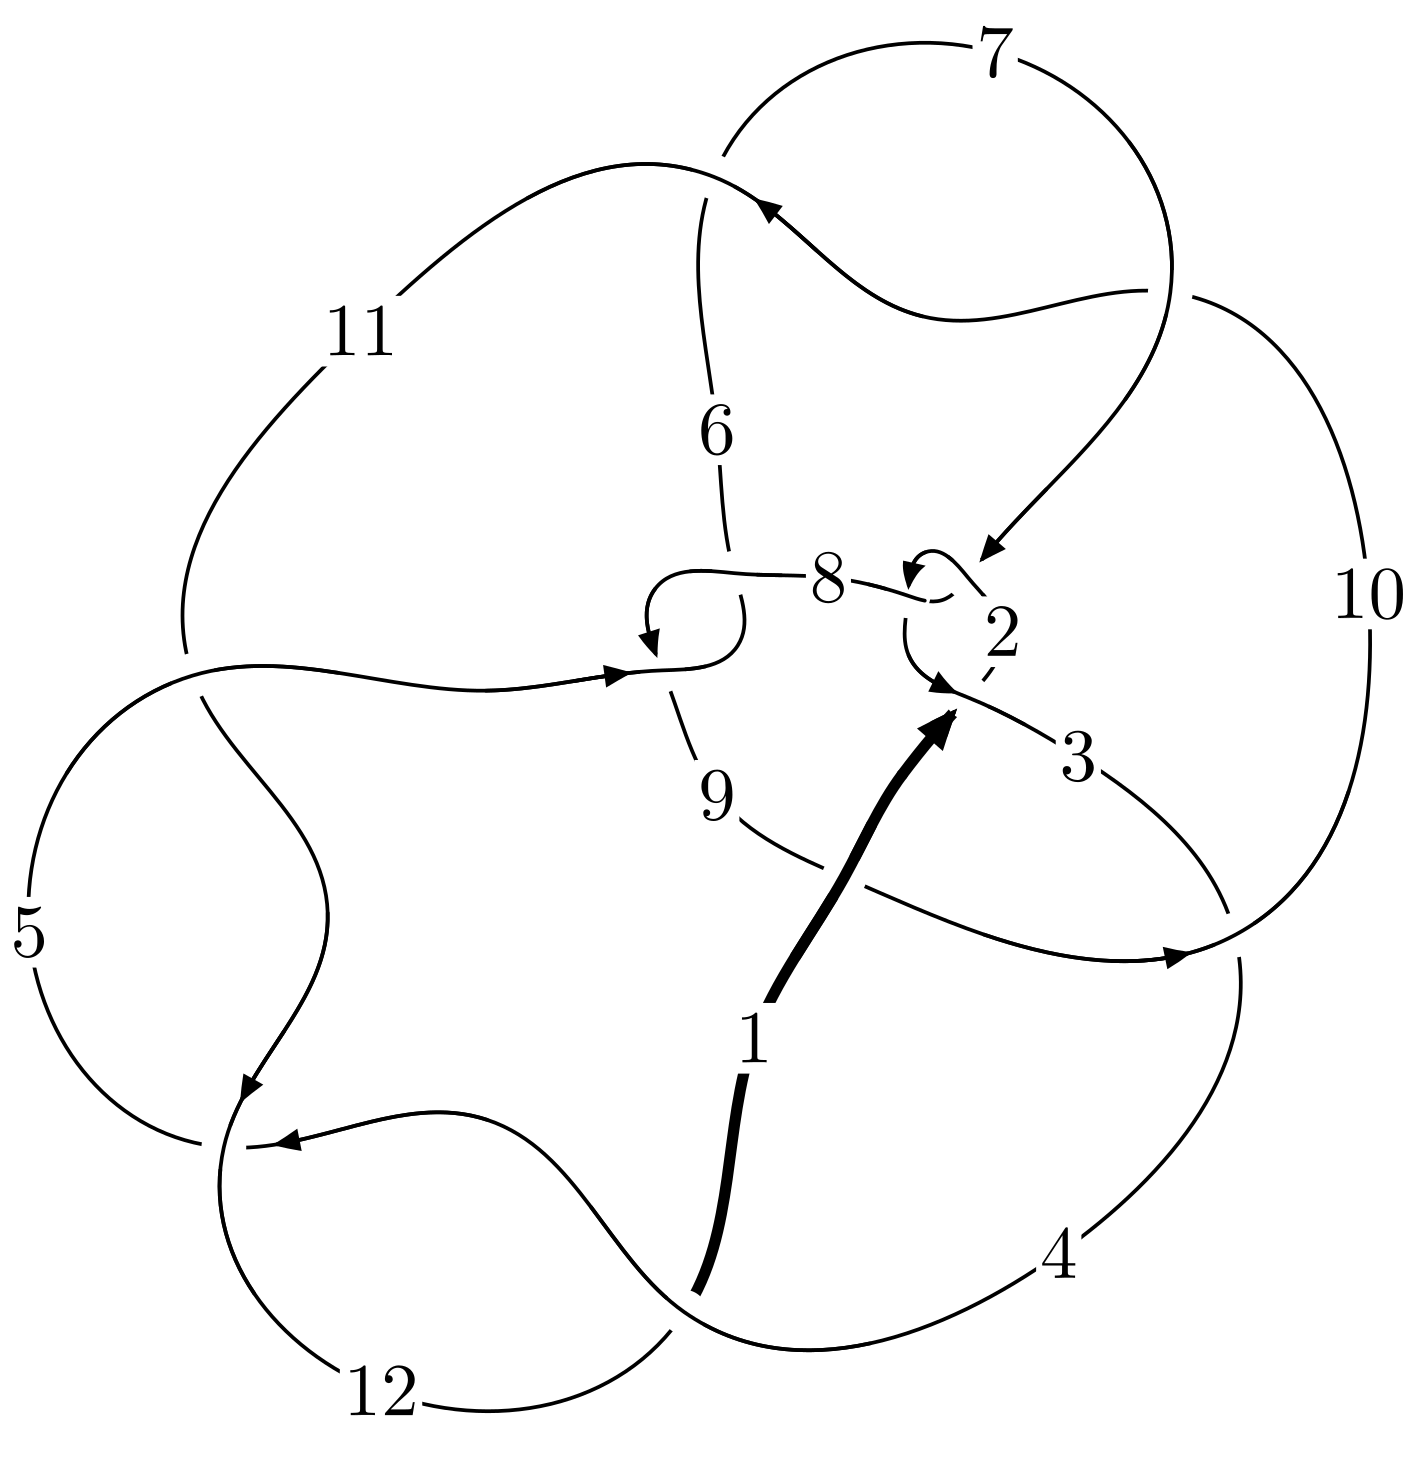
\includegraphics[width=112pt]{../../../GIT/diagram.site/Diagrams/png/2745_12n_0656.png}\\
\ \ \ A knot diagram\footnotemark}&
\allowdisplaybreaks
\textbf{Linearized knot diagam} \\
\cline{2-2}
 &
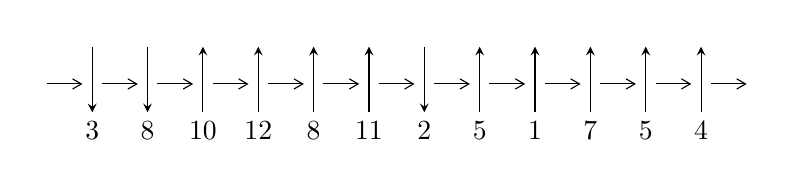
\begin{tikzpicture}[x=20pt, y=17pt]
	% nodes
	\node (C0) at (0, 0) {};
	\node (C1) at (1, 0) {};
	\node (C1U) at (1, +1) {};
	\node (C1D) at (1, -1) {3};

	\node (C2) at (2, 0) {};
	\node (C2U) at (2, +1) {};
	\node (C2D) at (2, -1) {8};

	\node (C3) at (3, 0) {};
	\node (C3U) at (3, +1) {};
	\node (C3D) at (3, -1) {10};

	\node (C4) at (4, 0) {};
	\node (C4U) at (4, +1) {};
	\node (C4D) at (4, -1) {12};

	\node (C5) at (5, 0) {};
	\node (C5U) at (5, +1) {};
	\node (C5D) at (5, -1) {8};

	\node (C6) at (6, 0) {};
	\node (C6U) at (6, +1) {};
	\node (C6D) at (6, -1) {11};

	\node (C7) at (7, 0) {};
	\node (C7U) at (7, +1) {};
	\node (C7D) at (7, -1) {2};

	\node (C8) at (8, 0) {};
	\node (C8U) at (8, +1) {};
	\node (C8D) at (8, -1) {5};

	\node (C9) at (9, 0) {};
	\node (C9U) at (9, +1) {};
	\node (C9D) at (9, -1) {1};

	\node (C10) at (10, 0) {};
	\node (C10U) at (10, +1) {};
	\node (C10D) at (10, -1) {7};

	\node (C11) at (11, 0) {};
	\node (C11U) at (11, +1) {};
	\node (C11D) at (11, -1) {5};

	\node (C12) at (12, 0) {};
	\node (C12U) at (12, +1) {};
	\node (C12D) at (12, -1) {4};
	\node (C13) at (13, 0) {};

	% arrows
	\draw[->,>={angle 60}]
	(C0) edge (C1) (C1) edge (C2) (C2) edge (C3) (C3) edge (C4) (C4) edge (C5) (C5) edge (C6) (C6) edge (C7) (C7) edge (C8) (C8) edge (C9) (C9) edge (C10) (C10) edge (C11) (C11) edge (C12) (C12) edge (C13) ;	\draw[->,>=stealth]
	(C1U) edge (C1D) (C2U) edge (C2D) (C3D) edge (C3U) (C4D) edge (C4U) (C5D) edge (C5U) (C6D) edge (C6U) (C7U) edge (C7D) (C8D) edge (C8U) (C9D) edge (C9U) (C10D) edge (C10U) (C11D) edge (C11U) (C12D) edge (C12U) ;
	\end{tikzpicture} \\
\hhline{~~} \\& 
\textbf{Solving Sequence} \\ \cline{2-2} 
 &
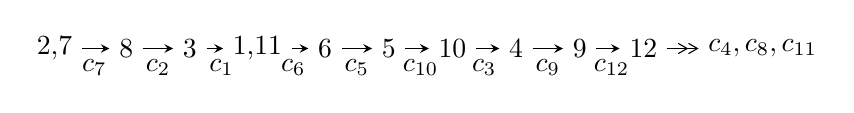
\begin{tikzpicture}[x=23pt, y=7pt]
	% node
	\node (A0) at (-1/8, 0) {2,7};
	\node (A1) at (1, 0) {8};
	\node (A2) at (2, 0) {3};
	\node (A3) at (49/16, 0) {1,11};
	\node (A4) at (33/8, 0) {6};
	\node (A5) at (41/8, 0) {5};
	\node (A6) at (49/8, 0) {10};
	\node (A7) at (57/8, 0) {4};
	\node (A8) at (65/8, 0) {9};
	\node (A9) at (73/8, 0) {12};
	\node (C1) at (1/2, -1) {$c_{7}$};
	\node (C2) at (3/2, -1) {$c_{2}$};
	\node (C3) at (5/2, -1) {$c_{1}$};
	\node (C4) at (29/8, -1) {$c_{6}$};
	\node (C5) at (37/8, -1) {$c_{5}$};
	\node (C6) at (45/8, -1) {$c_{10}$};
	\node (C7) at (53/8, -1) {$c_{3}$};
	\node (C8) at (61/8, -1) {$c_{9}$};
	\node (C9) at (69/8, -1) {$c_{12}$};
	\node (A10) at (11, 0) {$c_{4},c_{8},c_{11}$};

	% edge
	\draw[->,>=stealth]	
	(A0) edge (A1) (A1) edge (A2) (A2) edge (A3) (A3) edge (A4) (A4) edge (A5) (A5) edge (A6) (A6) edge (A7) (A7) edge (A8) (A8) edge (A9) ;
	\draw[->>,>={angle 60}]	
	(A9) edge (A10);
\end{tikzpicture} \\ 

\end{tabular} \\

\footnotetext{
The image of knot diagram is generated by the software ``\textbf{Draw programme}" developed by Andrew Bartholomew(\url{http://www.layer8.co.uk/maths/draw/index.htm\#Running-draw}), where we modified some parts for our purpose(\url{https://github.com/CATsTAILs/LinksPainter}).
}\phantom \\ \newline 
\centering \textbf{Ideals for irreducible components\footnotemark of $X_{\text{par}}$} 
 
\begin{align*}
I^u_{1}&=\langle 
-5.04974\times10^{93} u^{65}-9.74388\times10^{92} u^{64}+\cdots+4.92845\times10^{93} b+3.58696\times10^{95},\\
\phantom{I^u_{1}}&\phantom{= \langle  }2.17687\times10^{95} u^{65}-2.86390\times10^{95} u^{64}+\cdots+3.89347\times10^{95} a-3.06729\times10^{97},\;u^{66}- u^{65}+\cdots-51 u+79\rangle \\
I^u_{2}&=\langle 
u^{15}-4 u^{13}- u^{12}+8 u^{11}+5 u^{10}-8 u^9-13 u^8+3 u^7+21 u^6+u^5-19 u^4- u^3+7 u^2+b,\\
\phantom{I^u_{2}}&\phantom{= \langle  }-5 u^{16}+u^{15}+\cdots+a-1,\\
\phantom{I^u_{2}}&\phantom{= \langle  }u^{17}-4 u^{15}- u^{14}+9 u^{13}+5 u^{12}-11 u^{11}-14 u^{10}+8 u^9+25 u^8-2 u^7-28 u^6- u^5+19 u^4+u^3-7 u^2+1\rangle \\
\\
\end{align*}
\raggedright * 2 irreducible components of $\dim_{\mathbb{C}}=0$, with total 83 representations.\\
\footnotetext{All coefficients of polynomials are rational numbers. But the coefficients are sometimes approximated in decimal forms when there is not enough margin.}
\newpage
\renewcommand{\arraystretch}{1}
\centering \section*{I. $I^u_{1}= \langle -5.05\times10^{93} u^{65}-9.74\times10^{92} u^{64}+\cdots+4.93\times10^{93} b+3.59\times10^{95},\;2.18\times10^{95} u^{65}-2.86\times10^{95} u^{64}+\cdots+3.89\times10^{95} a-3.07\times10^{97},\;u^{66}- u^{65}+\cdots-51 u+79 \rangle$}
\flushleft \textbf{(i) Arc colorings}\\
\begin{tabular}{m{7pt} m{180pt} m{7pt} m{180pt} }
\flushright $a_{2}=$&$\begin{pmatrix}0\\u\end{pmatrix}$ \\
\flushright $a_{7}=$&$\begin{pmatrix}1\\0\end{pmatrix}$ \\
\flushright $a_{8}=$&$\begin{pmatrix}1\\u^2\end{pmatrix}$ \\
\flushright $a_{3}=$&$\begin{pmatrix}- u\\- u^3+u\end{pmatrix}$ \\
\flushright $a_{1}=$&$\begin{pmatrix}u^3\\u^5- u^3+u\end{pmatrix}$ \\
\flushright $a_{11}=$&$\begin{pmatrix}-0.559109 u^{65}+0.735565 u^{64}+\cdots+114.511 u+78.7804\\1.02461 u^{65}+0.197707 u^{64}+\cdots+26.4996 u-72.7807\end{pmatrix}$ \\
\flushright $a_{6}=$&$\begin{pmatrix}-2.35020 u^{65}+0.204588 u^{64}+\cdots+49.0040 u+156.891\\-2.94625 u^{65}+0.504266 u^{64}+\cdots+106.949 u+284.585\end{pmatrix}$ \\
\flushright $a_{5}=$&$\begin{pmatrix}-1.48828 u^{65}+0.0869445 u^{64}+\cdots+18.2941 u+41.8085\\-2.60902 u^{65}+0.363501 u^{64}+\cdots+76.8159 u+225.788\end{pmatrix}$ \\
\flushright $a_{10}=$&$\begin{pmatrix}-1.58372 u^{65}+0.537858 u^{64}+\cdots+88.0118 u+151.561\\1.02461 u^{65}+0.197707 u^{64}+\cdots+26.4996 u-72.7807\end{pmatrix}$ \\
\flushright $a_{4}=$&$\begin{pmatrix}0.833366 u^{65}-0.878185 u^{64}+\cdots-147.529 u-89.3505\\-1.62313 u^{65}+0.338423 u^{64}+\cdots+76.6054 u+160.632\end{pmatrix}$ \\
\flushright $a_{9}=$&$\begin{pmatrix}-1.86117 u^{65}+0.899303 u^{64}+\cdots+144.315 u+201.743\\0.488512 u^{65}+0.502843 u^{64}+\cdots+75.8217 u-8.74372\end{pmatrix}$ \\
\flushright $a_{12}=$&$\begin{pmatrix}-0.606622 u^{65}-0.258104 u^{64}+\cdots-12.2197 u+16.0020\\-0.770254 u^{65}-0.0843692 u^{64}+\cdots-0.510519 u+38.6892\end{pmatrix}$\\&\end{tabular}
\flushleft \textbf{(ii) Obstruction class $= -1$}\\~\\
\flushleft \textbf{(iii) Cusp Shapes $= -4.68718 u^{65}+2.07367 u^{64}+\cdots+423.125 u+473.176$}\\~\\
\newpage\renewcommand{\arraystretch}{1}
\flushleft \textbf{(iv) u-Polynomials at the component}\newline \\
\begin{tabular}{m{50pt}|m{274pt}}
Crossings & \hspace{64pt}u-Polynomials at each crossing \\
\hline $$\begin{aligned}c_{1}\end{aligned}$$&$\begin{aligned}
&u^{66}+25 u^{65}+\cdots+108619 u+6241
\end{aligned}$\\
\hline $$\begin{aligned}c_{2},c_{7}\end{aligned}$$&$\begin{aligned}
&u^{66}+u^{65}+\cdots+51 u+79
\end{aligned}$\\
\hline $$\begin{aligned}c_{3}\end{aligned}$$&$\begin{aligned}
&u^{66}+u^{65}+\cdots-320 u-32
\end{aligned}$\\
\hline $$\begin{aligned}c_{4},c_{11},c_{12}\end{aligned}$$&$\begin{aligned}
&u^{66}+2 u^{65}+\cdots-135 u-19
\end{aligned}$\\
\hline $$\begin{aligned}c_{5},c_{8}\end{aligned}$$&$\begin{aligned}
&u^{66}+6 u^{65}+\cdots+256 u-112
\end{aligned}$\\
\hline $$\begin{aligned}c_{6},c_{10}\end{aligned}$$&$\begin{aligned}
&u^{66}- u^{65}+\cdots-22 u-1
\end{aligned}$\\
\hline $$\begin{aligned}c_{9}\end{aligned}$$&$\begin{aligned}
&u^{66}+u^{65}+\cdots+9183 u+1252
\end{aligned}$\\
\hline
\end{tabular}\\~\\
\newpage\renewcommand{\arraystretch}{1}
\flushleft \textbf{(v) Riley Polynomials at the component}\newline \\
\begin{tabular}{m{50pt}|m{274pt}}
Crossings & \hspace{64pt}Riley Polynomials at each crossing \\
\hline $$\begin{aligned}c_{1}\end{aligned}$$&$\begin{aligned}
&y^{66}+35 y^{65}+\cdots-251925111 y+38950081
\end{aligned}$\\
\hline $$\begin{aligned}c_{2},c_{7}\end{aligned}$$&$\begin{aligned}
&y^{66}-25 y^{65}+\cdots-108619 y+6241
\end{aligned}$\\
\hline $$\begin{aligned}c_{3}\end{aligned}$$&$\begin{aligned}
&y^{66}+27 y^{65}+\cdots-115712 y+1024
\end{aligned}$\\
\hline $$\begin{aligned}c_{4},c_{11},c_{12}\end{aligned}$$&$\begin{aligned}
&y^{66}+56 y^{65}+\cdots-7357 y+361
\end{aligned}$\\
\hline $$\begin{aligned}c_{5},c_{8}\end{aligned}$$&$\begin{aligned}
&y^{66}-50 y^{65}+\cdots-1254528 y+12544
\end{aligned}$\\
\hline $$\begin{aligned}c_{6},c_{10}\end{aligned}$$&$\begin{aligned}
&y^{66}+11 y^{65}+\cdots-78 y+1
\end{aligned}$\\
\hline $$\begin{aligned}c_{9}\end{aligned}$$&$\begin{aligned}
&y^{66}-13 y^{65}+\cdots-59172305 y+1567504
\end{aligned}$\\
\hline
\end{tabular}\\~\\
\newpage\flushleft \textbf{(vi) Complex Volumes and Cusp Shapes}
$$\begin{array}{c|c|c}  
\text{Solutions to }I^u_{1}& \I (\text{vol} + \sqrt{-1}CS) & \text{Cusp shape}\\
 \hline 
\begin{aligned}
u &= -0.257112 + 0.947624 I \\
a &= \phantom{-}0.071468 - 0.219305 I \\
b &= -0.934003 - 0.145624 I\end{aligned}
 & \phantom{-}0.1053660 + 0.0685567 I & \phantom{-}6.00000 + 0. I\phantom{ +0.000000I} \\ \hline\begin{aligned}
u &= -0.257112 - 0.947624 I \\
a &= \phantom{-}0.071468 + 0.219305 I \\
b &= -0.934003 + 0.145624 I\end{aligned}
 & \phantom{-}0.1053660 - 0.0685567 I & \phantom{-}6.00000 + 0. I\phantom{ +0.000000I} \\ \hline\begin{aligned}
u &= \phantom{-}0.707502 + 0.680828 I \\
a &= \phantom{-}0.510614 + 0.653841 I \\
b &= -0.410733 + 0.515754 I\end{aligned}
 & \phantom{-}0.03346 - 2.05159 I & \phantom{-}6.00000 + 4.98115 I \\ \hline\begin{aligned}
u &= \phantom{-}0.707502 - 0.680828 I \\
a &= \phantom{-}0.510614 - 0.653841 I \\
b &= -0.410733 - 0.515754 I\end{aligned}
 & \phantom{-}0.03346 + 2.05159 I & \phantom{-}6.00000 - 4.98115 I \\ \hline\begin{aligned}
u &= -0.775544 + 0.661698 I \\
a &= -0.65118 + 2.11101 I \\
b &= \phantom{-}1.02196 + 1.17957 I\end{aligned}
 & \phantom{-}0.84171 - 1.91050 I & \phantom{-}6.00000 + 0. I\phantom{ +0.000000I} \\ \hline\begin{aligned}
u &= -0.775544 - 0.661698 I \\
a &= -0.65118 - 2.11101 I \\
b &= \phantom{-}1.02196 - 1.17957 I\end{aligned}
 & \phantom{-}0.84171 + 1.91050 I & \phantom{-}6.00000 + 0. I\phantom{ +0.000000I} \\ \hline\begin{aligned}
u &= \phantom{-}0.855134 + 0.471238 I \\
a &= \phantom{-}0.28210 + 2.12553 I \\
b &= \phantom{-}0.203001 + 1.196910 I\end{aligned}
 & -6.43277 - 1.93176 I & \phantom{-0.000000 -}0. + 3.96327 I \\ \hline\begin{aligned}
u &= \phantom{-}0.855134 - 0.471238 I \\
a &= \phantom{-}0.28210 - 2.12553 I \\
b &= \phantom{-}0.203001 - 1.196910 I\end{aligned}
 & -6.43277 + 1.93176 I & \phantom{-0.000000 } 0. - 3.96327 I \\ \hline\begin{aligned}
u &= -0.695152 + 0.756763 I \\
a &= -0.285265 + 0.382734 I \\
b &= -1.096470 + 0.816570 I\end{aligned}
 & \phantom{-}2.92421 - 2.75395 I & \phantom{-}6.00000 + 0. I\phantom{ +0.000000I} \\ \hline\begin{aligned}
u &= -0.695152 - 0.756763 I \\
a &= -0.285265 - 0.382734 I \\
b &= -1.096470 - 0.816570 I\end{aligned}
 & \phantom{-}2.92421 + 2.75395 I & \phantom{-}6.00000 + 0. I\phantom{ +0.000000I}\\
 \hline 
 \end{array}$$\newpage$$\begin{array}{c|c|c}  
\text{Solutions to }I^u_{1}& \I (\text{vol} + \sqrt{-1}CS) & \text{Cusp shape}\\
 \hline 
\begin{aligned}
u &= -0.832084 + 0.479093 I \\
a &= -0.964406 - 0.722252 I \\
b &= \phantom{-}0.388483 + 0.305721 I\end{aligned}
 & -6.35326 + 1.92286 I & \phantom{-}0.61610 - 3.80019 I \\ \hline\begin{aligned}
u &= -0.832084 - 0.479093 I \\
a &= -0.964406 + 0.722252 I \\
b &= \phantom{-}0.388483 - 0.305721 I\end{aligned}
 & -6.35326 - 1.92286 I & \phantom{-}0.61610 + 3.80019 I \\ \hline\begin{aligned}
u &= \phantom{-}0.831367 + 0.696653 I \\
a &= -0.595869 - 0.242192 I \\
b &= -1.29532 - 0.88221 I\end{aligned}
 & \phantom{-}5.68298 - 2.17633 I & \phantom{-0.000000 } 0 \\ \hline\begin{aligned}
u &= \phantom{-}0.831367 - 0.696653 I \\
a &= -0.595869 + 0.242192 I \\
b &= -1.29532 + 0.88221 I\end{aligned}
 & \phantom{-}5.68298 + 2.17633 I & \phantom{-0.000000 } 0 \\ \hline\begin{aligned}
u &= \phantom{-}0.887020 + 0.687260 I \\
a &= -0.53117 - 2.06451 I \\
b &= \phantom{-}0.94726 - 1.09875 I\end{aligned}
 & \phantom{-}5.51025 - 3.14310 I & \phantom{-0.000000 } 0 \\ \hline\begin{aligned}
u &= \phantom{-}0.887020 - 0.687260 I \\
a &= -0.53117 + 2.06451 I \\
b &= \phantom{-}0.94726 + 1.09875 I\end{aligned}
 & \phantom{-}5.51025 + 3.14310 I & \phantom{-0.000000 } 0 \\ \hline\begin{aligned}
u &= \phantom{-}0.839142 + 0.235261 I \\
a &= \phantom{-}0.610217 + 0.679297 I \\
b &= -1.303620 + 0.043632 I\end{aligned}
 & -2.21197 + 2.72682 I & -0.929885 + 0.873234 I \\ \hline\begin{aligned}
u &= \phantom{-}0.839142 - 0.235261 I \\
a &= \phantom{-}0.610217 - 0.679297 I \\
b &= -1.303620 - 0.043632 I\end{aligned}
 & -2.21197 - 2.72682 I & -0.929885 - 0.873234 I \\ \hline\begin{aligned}
u &= -0.928111 + 0.642178 I \\
a &= -0.913757 + 0.186542 I \\
b &= -1.43369 + 1.01259 I\end{aligned}
 & \phantom{-}0.36496 + 6.98411 I & \phantom{-0.000000 } 0 \\ \hline\begin{aligned}
u &= -0.928111 - 0.642178 I \\
a &= -0.913757 - 0.186542 I \\
b &= -1.43369 - 1.01259 I\end{aligned}
 & \phantom{-}0.36496 - 6.98411 I & \phantom{-0.000000 } 0\\
 \hline 
 \end{array}$$\newpage$$\begin{array}{c|c|c}  
\text{Solutions to }I^u_{1}& \I (\text{vol} + \sqrt{-1}CS) & \text{Cusp shape}\\
 \hline 
\begin{aligned}
u &= \phantom{-}0.838382 + 0.213695 I \\
a &= -1.40107 - 2.19862 I \\
b &= \phantom{-}0.09948 - 1.79877 I\end{aligned}
 & -11.89330 - 0.93560 I & -4.33716 - 3.52776 I \\ \hline\begin{aligned}
u &= \phantom{-}0.838382 - 0.213695 I \\
a &= -1.40107 + 2.19862 I \\
b &= \phantom{-}0.09948 + 1.79877 I\end{aligned}
 & -11.89330 + 0.93560 I & -4.33716 + 3.52776 I \\ \hline\begin{aligned}
u &= -0.899982 + 0.708778 I \\
a &= \phantom{-}1.09863 - 0.90483 I \\
b &= -0.16265 - 1.57424 I\end{aligned}
 & -9.01530 + 2.75120 I & \phantom{-0.000000 } 0 \\ \hline\begin{aligned}
u &= -0.899982 - 0.708778 I \\
a &= \phantom{-}1.09863 + 0.90483 I \\
b &= -0.16265 + 1.57424 I\end{aligned}
 & -9.01530 - 2.75120 I & \phantom{-0.000000 } 0 \\ \hline\begin{aligned}
u &= \phantom{-}0.526272 + 1.019400 I \\
a &= \phantom{-}0.318206 + 0.066951 I \\
b &= \phantom{-}1.05853 + 0.95213 I\end{aligned}
 & \phantom{-}1.45735 + 9.54908 I & \phantom{-0.000000 } 0 \\ \hline\begin{aligned}
u &= \phantom{-}0.526272 - 1.019400 I \\
a &= \phantom{-}0.318206 - 0.066951 I \\
b &= \phantom{-}1.05853 - 0.95213 I\end{aligned}
 & \phantom{-}1.45735 - 9.54908 I & \phantom{-0.000000 } 0 \\ \hline\begin{aligned}
u &= -1.102590 + 0.320589 I \\
a &= \phantom{-}0.33068 - 1.61344 I \\
b &= \phantom{-}0.266522 - 0.929330 I\end{aligned}
 & -6.22093 + 0.10686 I & \phantom{-0.000000 } 0 \\ \hline\begin{aligned}
u &= -1.102590 - 0.320589 I \\
a &= \phantom{-}0.33068 + 1.61344 I \\
b &= \phantom{-}0.266522 + 0.929330 I\end{aligned}
 & -6.22093 - 0.10686 I & \phantom{-0.000000 } 0 \\ \hline\begin{aligned}
u &= -0.834282 + 0.117518 I \\
a &= -0.44582 - 2.20169 I \\
b &= \phantom{-}0.106930 - 1.272370 I\end{aligned}
 & -4.82653 + 0.53157 I & \phantom{-}0.07384 + 2.64833 I \\ \hline\begin{aligned}
u &= -0.834282 - 0.117518 I \\
a &= -0.44582 + 2.20169 I \\
b &= \phantom{-}0.106930 + 1.272370 I\end{aligned}
 & -4.82653 - 0.53157 I & \phantom{-}0.07384 - 2.64833 I\\
 \hline 
 \end{array}$$\newpage$$\begin{array}{c|c|c}  
\text{Solutions to }I^u_{1}& \I (\text{vol} + \sqrt{-1}CS) & \text{Cusp shape}\\
 \hline 
\begin{aligned}
u &= -0.636597 + 1.006470 I \\
a &= \phantom{-}0.458947 - 0.050429 I \\
b &= \phantom{-}0.998665 - 0.921408 I\end{aligned}
 & \phantom{-}6.05616 - 4.04965 I & \phantom{-0.000000 } 0 \\ \hline\begin{aligned}
u &= -0.636597 - 1.006470 I \\
a &= \phantom{-}0.458947 + 0.050429 I \\
b &= \phantom{-}0.998665 + 0.921408 I\end{aligned}
 & \phantom{-}6.05616 + 4.04965 I & \phantom{-0.000000 } 0 \\ \hline\begin{aligned}
u &= -0.983398 + 0.684141 I \\
a &= -0.51377 + 2.02937 I \\
b &= \phantom{-}0.849833 + 1.042050 I\end{aligned}
 & \phantom{-}2.05072 + 8.22966 I & \phantom{-0.000000 } 0 \\ \hline\begin{aligned}
u &= -0.983398 - 0.684141 I \\
a &= -0.51377 - 2.02937 I \\
b &= \phantom{-}0.849833 - 1.042050 I\end{aligned}
 & \phantom{-}2.05072 - 8.22966 I & \phantom{-0.000000 } 0 \\ \hline\begin{aligned}
u &= \phantom{-}0.977568 + 0.708124 I \\
a &= -0.209781 - 0.209812 I \\
b &= \phantom{-}0.606595 - 0.224505 I\end{aligned}
 & -0.90500 - 3.33318 I & \phantom{-0.000000 } 0 \\ \hline\begin{aligned}
u &= \phantom{-}0.977568 - 0.708124 I \\
a &= -0.209781 + 0.209812 I \\
b &= \phantom{-}0.606595 + 0.224505 I\end{aligned}
 & -0.90500 + 3.33318 I & \phantom{-0.000000 } 0 \\ \hline\begin{aligned}
u &= \phantom{-}1.096460 + 0.507389 I \\
a &= -1.14935 - 1.39168 I \\
b &= \phantom{-}0.501177 - 0.634307 I\end{aligned}
 & -4.99940 - 7.29186 I & \phantom{-0.000000 } 0 \\ \hline\begin{aligned}
u &= \phantom{-}1.096460 - 0.507389 I \\
a &= -1.14935 + 1.39168 I \\
b &= \phantom{-}0.501177 + 0.634307 I\end{aligned}
 & -4.99940 + 7.29186 I & \phantom{-0.000000 } 0 \\ \hline\begin{aligned}
u &= -1.096320 + 0.542363 I \\
a &= -0.483047 + 1.273850 I \\
b &= \phantom{-}0.710209 + 0.578523 I\end{aligned}
 & -1.06694 + 5.17758 I & \phantom{-0.000000 } 0 \\ \hline\begin{aligned}
u &= -1.096320 - 0.542363 I \\
a &= -0.483047 - 1.273850 I \\
b &= \phantom{-}0.710209 - 0.578523 I\end{aligned}
 & -1.06694 - 5.17758 I & \phantom{-0.000000 } 0\\
 \hline 
 \end{array}$$\newpage$$\begin{array}{c|c|c}  
\text{Solutions to }I^u_{1}& \I (\text{vol} + \sqrt{-1}CS) & \text{Cusp shape}\\
 \hline 
\begin{aligned}
u &= \phantom{-}0.764652 + 0.955944 I \\
a &= \phantom{-}0.586188 + 0.078330 I \\
b &= \phantom{-}0.846583 + 0.894829 I\end{aligned}
 & \phantom{-}2.53161 - 1.78458 I & \phantom{-0.000000 } 0 \\ \hline\begin{aligned}
u &= \phantom{-}0.764652 - 0.955944 I \\
a &= \phantom{-}0.586188 - 0.078330 I \\
b &= \phantom{-}0.846583 - 0.894829 I\end{aligned}
 & \phantom{-}2.53161 + 1.78458 I & \phantom{-0.000000 } 0 \\ \hline\begin{aligned}
u &= \phantom{-}0.393732 + 1.163820 I \\
a &= \phantom{-}0.284564 + 0.124345 I \\
b &= \phantom{-}0.243672 + 0.002661 I\end{aligned}
 & \phantom{-}0.89352 - 2.40317 I & \phantom{-0.000000 } 0 \\ \hline\begin{aligned}
u &= \phantom{-}0.393732 - 1.163820 I \\
a &= \phantom{-}0.284564 - 0.124345 I \\
b &= \phantom{-}0.243672 - 0.002661 I\end{aligned}
 & \phantom{-}0.89352 + 2.40317 I & \phantom{-0.000000 } 0 \\ \hline\begin{aligned}
u &= \phantom{-}0.763441 + 0.052004 I \\
a &= \phantom{-}2.67743 + 1.41213 I \\
b &= \phantom{-}0.283142 + 0.043659 I\end{aligned}
 & -2.06277 + 3.79226 I & -1.58367 - 5.91104 I \\ \hline\begin{aligned}
u &= \phantom{-}0.763441 - 0.052004 I \\
a &= \phantom{-}2.67743 - 1.41213 I \\
b &= \phantom{-}0.283142 - 0.043659 I\end{aligned}
 & -2.06277 - 3.79226 I & -1.58367 + 5.91104 I \\ \hline\begin{aligned}
u &= \phantom{-}1.237200 + 0.275538 I \\
a &= -0.149817 + 1.097540 I \\
b &= -0.115179 + 0.814116 I\end{aligned}
 & -2.61077 - 2.63613 I & \phantom{-0.000000 } 0 \\ \hline\begin{aligned}
u &= \phantom{-}1.237200 - 0.275538 I \\
a &= -0.149817 - 1.097540 I \\
b &= -0.115179 - 0.814116 I\end{aligned}
 & -2.61077 + 2.63613 I & \phantom{-0.000000 } 0 \\ \hline\begin{aligned}
u &= -0.728667\phantom{ +0.000000I} \\
a &= \phantom{-}2.69016\phantom{ +0.000000I} \\
b &= \phantom{-}0.228552\phantom{ +0.000000I}\end{aligned}
 & \phantom{-}1.95571\phantom{ +0.000000I} & \phantom{-}2.70420\phantom{ +0.000000I} \\ \hline\begin{aligned}
u &= \phantom{-}1.211310 + 0.434932 I \\
a &= \phantom{-}0.216289 - 1.388270 I \\
b &= \phantom{-}0.908237 - 0.547503 I\end{aligned}
 & -4.31364 - 4.41545 I & \phantom{-0.000000 } 0\\
 \hline 
 \end{array}$$\newpage$$\begin{array}{c|c|c}  
\text{Solutions to }I^u_{1}& \I (\text{vol} + \sqrt{-1}CS) & \text{Cusp shape}\\
 \hline 
\begin{aligned}
u &= \phantom{-}1.211310 - 0.434932 I \\
a &= \phantom{-}0.216289 + 1.388270 I \\
b &= \phantom{-}0.908237 + 0.547503 I\end{aligned}
 & -4.31364 + 4.41545 I & \phantom{-0.000000 } 0 \\ \hline\begin{aligned}
u &= -0.368903 + 0.599292 I \\
a &= \phantom{-}0.551631 + 0.006032 I \\
b &= -0.543091 + 0.225358 I\end{aligned}
 & \phantom{-}1.044430 - 0.587332 I & \phantom{-}8.98331 + 3.47323 I \\ \hline\begin{aligned}
u &= -0.368903 - 0.599292 I \\
a &= \phantom{-}0.551631 - 0.006032 I \\
b &= -0.543091 - 0.225358 I\end{aligned}
 & \phantom{-}1.044430 + 0.587332 I & \phantom{-}8.98331 - 3.47323 I \\ \hline\begin{aligned}
u &= \phantom{-}1.028890 + 0.791131 I \\
a &= \phantom{-}0.45447 + 1.39568 I \\
b &= -0.90585 + 1.21148 I\end{aligned}
 & \phantom{-}1.64235 - 4.60831 I & \phantom{-0.000000 } 0 \\ \hline\begin{aligned}
u &= \phantom{-}1.028890 - 0.791131 I \\
a &= \phantom{-}0.45447 - 1.39568 I \\
b &= -0.90585 - 1.21148 I\end{aligned}
 & \phantom{-}1.64235 + 4.60831 I & \phantom{-0.000000 } 0 \\ \hline\begin{aligned}
u &= \phantom{-}0.192509 + 0.631326 I \\
a &= \phantom{-}1.095920 - 0.610070 I \\
b &= -0.227382 - 0.678722 I\end{aligned}
 & -2.56446 + 2.95191 I & \phantom{-}1.85269 - 4.42524 I \\ \hline\begin{aligned}
u &= \phantom{-}0.192509 - 0.631326 I \\
a &= \phantom{-}1.095920 + 0.610070 I \\
b &= -0.227382 + 0.678722 I\end{aligned}
 & -2.56446 - 2.95191 I & \phantom{-}1.85269 + 4.42524 I \\ \hline\begin{aligned}
u &= -1.110370 + 0.768499 I \\
a &= \phantom{-}0.37175 - 1.58877 I \\
b &= -1.04037 - 1.21889 I\end{aligned}
 & \phantom{-}4.54605 + 10.49520 I & \phantom{-0.000000 } 0 \\ \hline\begin{aligned}
u &= -1.110370 - 0.768499 I \\
a &= \phantom{-}0.37175 + 1.58877 I \\
b &= -1.04037 + 1.21889 I\end{aligned}
 & \phantom{-}4.54605 - 10.49520 I & \phantom{-0.000000 } 0 \\ \hline\begin{aligned}
u &= -0.639532\phantom{ +0.000000I} \\
a &= \phantom{-}0.572453\phantom{ +0.000000I} \\
b &= -1.15533\phantom{ +0.000000I}\end{aligned}
 & \phantom{-}2.36942\phantom{ +0.000000I} & -1.84080\phantom{ +0.000000I}\\
 \hline 
 \end{array}$$\newpage$$\begin{array}{c|c|c}  
\text{Solutions to }I^u_{1}& \I (\text{vol} + \sqrt{-1}CS) & \text{Cusp shape}\\
 \hline 
\begin{aligned}
u &= \phantom{-}1.156750 + 0.728414 I \\
a &= \phantom{-}0.35107 + 1.71491 I \\
b &= -1.10396 + 1.21839 I\end{aligned}
 & -0.5174 - 15.8754 I & \phantom{-0.000000 } 0 \\ \hline\begin{aligned}
u &= \phantom{-}1.156750 - 0.728414 I \\
a &= \phantom{-}0.35107 - 1.71491 I \\
b &= -1.10396 - 1.21839 I\end{aligned}
 & -0.5174 + 15.8754 I & \phantom{-0.000000 } 0 \\ \hline\begin{aligned}
u &= -1.396300 + 0.095553 I \\
a &= -0.539554 - 0.929625 I \\
b &= -0.390433 - 0.822365 I\end{aligned}
 & -6.23593 + 6.65763 I & \phantom{-0.000000 } 0 \\ \hline\begin{aligned}
u &= -1.396300 - 0.095553 I \\
a &= -0.539554 + 0.929625 I \\
b &= -0.390433 + 0.822365 I\end{aligned}
 & -6.23593 - 6.65763 I & \phantom{-0.000000 } 0 \\ \hline\begin{aligned}
u &= -1.206480 + 0.716734 I \\
a &= \phantom{-}0.198206 + 0.687413 I \\
b &= \phantom{-}0.885867 + 0.292505 I\end{aligned}
 & -2.62837 + 5.98510 I & \phantom{-0.000000 } 0 \\ \hline\begin{aligned}
u &= -1.206480 - 0.716734 I \\
a &= \phantom{-}0.198206 - 0.687413 I \\
b &= \phantom{-}0.885867 - 0.292505 I\end{aligned}
 & -2.62837 - 5.98510 I & \phantom{-0.000000 } 0\\
 \hline 
 \end{array}$$\newpage\newpage\renewcommand{\arraystretch}{1}
\centering \section*{II. $I^u_{2}= \langle u^{15}-4 u^{13}+\cdots+7 u^2+b,\;-5 u^{16}+u^{15}+\cdots+a-1,\;u^{17}-4 u^{15}+\cdots-7 u^2+1 \rangle$}
\flushleft \textbf{(i) Arc colorings}\\
\begin{tabular}{m{7pt} m{180pt} m{7pt} m{180pt} }
\flushright $a_{2}=$&$\begin{pmatrix}0\\u\end{pmatrix}$ \\
\flushright $a_{7}=$&$\begin{pmatrix}1\\0\end{pmatrix}$ \\
\flushright $a_{8}=$&$\begin{pmatrix}1\\u^2\end{pmatrix}$ \\
\flushright $a_{3}=$&$\begin{pmatrix}- u\\- u^3+u\end{pmatrix}$ \\
\flushright $a_{1}=$&$\begin{pmatrix}u^3\\u^5- u^3+u\end{pmatrix}$ \\
\flushright $a_{11}=$&$\begin{pmatrix}5 u^{16}- u^{15}+\cdots-6 u+1\\- u^{15}+4 u^{13}+\cdots+u^3-7 u^2\end{pmatrix}$ \\
\flushright $a_{6}=$&$\begin{pmatrix}- u^{15}- u^{14}+\cdots-27 u^2+4\\2 u^{15}- u^{14}+\cdots- u+2\end{pmatrix}$ \\
\flushright $a_{5}=$&$\begin{pmatrix}- u^{16}- u^{15}+\cdots+u+3\\- u^{16}+2 u^{15}+\cdots-4 u^2+2\end{pmatrix}$ \\
\flushright $a_{10}=$&$\begin{pmatrix}5 u^{16}-16 u^{14}+\cdots-6 u+1\\- u^{15}+4 u^{13}+\cdots+u^3-7 u^2\end{pmatrix}$ \\
\flushright $a_{4}=$&$\begin{pmatrix}7 u^{15}-25 u^{13}+\cdots+66 u^2-12\\u^{14}-3 u^{12}- u^{11}+5 u^{10}+4 u^9-3 u^8-9 u^7+12 u^5+u^4-8 u^3+u\end{pmatrix}$ \\
\flushright $a_{9}=$&$\begin{pmatrix}7 u^{16}- u^{15}+\cdots-9 u+2\\2 u^{16}- u^{15}+\cdots-5 u^2-3 u\end{pmatrix}$ \\
\flushright $a_{12}=$&$\begin{pmatrix}-4 u^{16}+17 u^{14}+\cdots+13 u+4\\-2 u^{16}+2 u^{15}+\cdots+3 u-5\end{pmatrix}$\\&\end{tabular}
\flushleft \textbf{(ii) Obstruction class $= 1$}\\~\\
\flushleft \textbf{(iii) Cusp Shapes $= 16 u^{16}-15 u^{15}-53 u^{14}+38 u^{13}+120 u^{12}-41 u^{11}-166 u^{10}-61 u^9+228 u^8+210 u^7-284 u^6-240 u^5+269 u^4+129 u^3-141 u^2-24 u+36$}\\~\\
\newpage\renewcommand{\arraystretch}{1}
\flushleft \textbf{(iv) u-Polynomials at the component}\newline \\
\begin{tabular}{m{50pt}|m{274pt}}
Crossings & \hspace{64pt}u-Polynomials at each crossing \\
\hline $$\begin{aligned}c_{1}\end{aligned}$$&$\begin{aligned}
&u^{17}-8 u^{16}+\cdots+14 u-1
\end{aligned}$\\
\hline $$\begin{aligned}c_{2}\end{aligned}$$&$\begin{aligned}
&u^{17}-4 u^{15}+\cdots+7 u^2-1
\end{aligned}$\\
\hline $$\begin{aligned}c_{3}\end{aligned}$$&$\begin{aligned}
&u^{17}+8 u^{15}+\cdots-6 u^2-1
\end{aligned}$\\
\hline $$\begin{aligned}c_{4}\end{aligned}$$&$\begin{aligned}
&u^{17}- u^{16}+\cdots-10 u^2-1
\end{aligned}$\\
\hline $$\begin{aligned}c_{5}\end{aligned}$$&$\begin{aligned}
&u^{17}+u^{16}+\cdots+6 u^2+1
\end{aligned}$\\
\hline $$\begin{aligned}c_{6}\end{aligned}$$&$\begin{aligned}
&u^{17}+6 u^{15}+\cdots+u+1
\end{aligned}$\\
\hline $$\begin{aligned}c_{7}\end{aligned}$$&$\begin{aligned}
&u^{17}-4 u^{15}+\cdots-7 u^2+1
\end{aligned}$\\
\hline $$\begin{aligned}c_{8}\end{aligned}$$&$\begin{aligned}
&u^{17}- u^{16}+\cdots-6 u^2-1
\end{aligned}$\\
\hline $$\begin{aligned}c_{9}\end{aligned}$$&$\begin{aligned}
&u^{17}-2 u^{15}+\cdots+4 u+13
\end{aligned}$\\
\hline $$\begin{aligned}c_{10}\end{aligned}$$&$\begin{aligned}
&u^{17}+6 u^{15}+\cdots+u-1
\end{aligned}$\\
\hline $$\begin{aligned}c_{11},c_{12}\end{aligned}$$&$\begin{aligned}
&u^{17}+u^{16}+\cdots+10 u^2+1
\end{aligned}$\\
\hline
\end{tabular}\\~\\
\newpage\renewcommand{\arraystretch}{1}
\flushleft \textbf{(v) Riley Polynomials at the component}\newline \\
\begin{tabular}{m{50pt}|m{274pt}}
Crossings & \hspace{64pt}Riley Polynomials at each crossing \\
\hline $$\begin{aligned}c_{1}\end{aligned}$$&$\begin{aligned}
&y^{17}+4 y^{16}+\cdots+22 y-1
\end{aligned}$\\
\hline $$\begin{aligned}c_{2},c_{7}\end{aligned}$$&$\begin{aligned}
&y^{17}-8 y^{16}+\cdots+14 y-1
\end{aligned}$\\
\hline $$\begin{aligned}c_{3}\end{aligned}$$&$\begin{aligned}
&y^{17}+16 y^{16}+\cdots-12 y-1
\end{aligned}$\\
\hline $$\begin{aligned}c_{4},c_{11},c_{12}\end{aligned}$$&$\begin{aligned}
&y^{17}+21 y^{16}+\cdots-20 y-1
\end{aligned}$\\
\hline $$\begin{aligned}c_{5},c_{8}\end{aligned}$$&$\begin{aligned}
&y^{17}-5 y^{16}+\cdots-12 y-1
\end{aligned}$\\
\hline $$\begin{aligned}c_{6},c_{10}\end{aligned}$$&$\begin{aligned}
&y^{17}+12 y^{16}+\cdots+5 y-1
\end{aligned}$\\
\hline $$\begin{aligned}c_{9}\end{aligned}$$&$\begin{aligned}
&y^{17}-4 y^{16}+\cdots+276 y-169
\end{aligned}$\\
\hline
\end{tabular}\\~\\
\newpage\flushleft \textbf{(vi) Complex Volumes and Cusp Shapes}
$$\begin{array}{c|c|c}  
\text{Solutions to }I^u_{2}& \I (\text{vol} + \sqrt{-1}CS) & \text{Cusp shape}\\
 \hline 
\begin{aligned}
u &= -0.935454 + 0.285621 I \\
a &= -0.74965 - 2.16184 I \\
b &= \phantom{-}0.134278 - 0.894052 I\end{aligned}
 & -7.54669 + 1.17742 I & -6.67270 - 0.38814 I \\ \hline\begin{aligned}
u &= -0.935454 - 0.285621 I \\
a &= -0.74965 + 2.16184 I \\
b &= \phantom{-}0.134278 + 0.894052 I\end{aligned}
 & -7.54669 - 1.17742 I & -6.67270 + 0.38814 I \\ \hline\begin{aligned}
u &= \phantom{-}0.912131 + 0.328638 I \\
a &= \phantom{-}0.30968 + 2.00614 I \\
b &= \phantom{-}0.147743 + 1.270230 I\end{aligned}
 & -4.60840 - 1.36971 I & \phantom{-}3.49419 + 5.08345 I \\ \hline\begin{aligned}
u &= \phantom{-}0.912131 - 0.328638 I \\
a &= \phantom{-}0.30968 - 2.00614 I \\
b &= \phantom{-}0.147743 - 1.270230 I\end{aligned}
 & -4.60840 + 1.36971 I & \phantom{-}3.49419 - 5.08345 I \\ \hline\begin{aligned}
u &= -0.889395 + 0.372697 I \\
a &= \phantom{-}1.29749 - 2.05795 I \\
b &= \phantom{-}0.11611 - 1.91684 I\end{aligned}
 & -11.58440 + 1.56045 I & \phantom{-}1.25948 - 6.47821 I \\ \hline\begin{aligned}
u &= -0.889395 - 0.372697 I \\
a &= \phantom{-}1.29749 + 2.05795 I \\
b &= \phantom{-}0.11611 + 1.91684 I\end{aligned}
 & -11.58440 - 1.56045 I & \phantom{-}1.25948 + 6.47821 I \\ \hline\begin{aligned}
u &= \phantom{-}0.938625 + 0.706892 I \\
a &= -1.030120 - 0.743145 I \\
b &= \phantom{-}0.181857 - 1.388630 I\end{aligned}
 & -9.53882 - 2.78092 I & -6.42091 + 3.83492 I \\ \hline\begin{aligned}
u &= \phantom{-}0.938625 - 0.706892 I \\
a &= -1.030120 + 0.743145 I \\
b &= \phantom{-}0.181857 + 1.388630 I\end{aligned}
 & -9.53882 + 2.78092 I & -6.42091 - 3.83492 I \\ \hline\begin{aligned}
u &= -0.430993 + 1.143370 I \\
a &= -0.247474 - 0.064001 I \\
b &= -0.515702 + 0.275227 I\end{aligned}
 & \phantom{-}0.99848 + 2.09379 I & \phantom{-}7.49851 + 6.90388 I \\ \hline\begin{aligned}
u &= -0.430993 - 1.143370 I \\
a &= -0.247474 + 0.064001 I \\
b &= -0.515702 - 0.275227 I\end{aligned}
 & \phantom{-}0.99848 - 2.09379 I & \phantom{-}7.49851 - 6.90388 I\\
 \hline 
 \end{array}$$\newpage$$\begin{array}{c|c|c}  
\text{Solutions to }I^u_{2}& \I (\text{vol} + \sqrt{-1}CS) & \text{Cusp shape}\\
 \hline 
\begin{aligned}
u &= \phantom{-}1.193420 + 0.475980 I \\
a &= -0.017645 - 1.033010 I \\
b &= \phantom{-}0.711571 - 0.148908 I\end{aligned}
 & -4.07323 - 6.22059 I & \phantom{-}1.13082 + 6.76795 I \\ \hline\begin{aligned}
u &= \phantom{-}1.193420 - 0.475980 I \\
a &= -0.017645 + 1.033010 I \\
b &= \phantom{-}0.711571 + 0.148908 I\end{aligned}
 & -4.07323 + 6.22059 I & \phantom{-}1.13082 - 6.76795 I \\ \hline\begin{aligned}
u &= -1.151330 + 0.648836 I \\
a &= -0.250827 + 0.900595 I \\
b &= \phantom{-}0.603765 + 0.579563 I\end{aligned}
 & -1.51682 + 4.20012 I & \phantom{-}2.90139 - 4.71038 I \\ \hline\begin{aligned}
u &= -1.151330 - 0.648836 I \\
a &= -0.250827 - 0.900595 I \\
b &= \phantom{-}0.603765 - 0.579563 I\end{aligned}
 & -1.51682 - 4.20012 I & \phantom{-}2.90139 + 4.71038 I \\ \hline\begin{aligned}
u &= \phantom{-}0.611850 + 0.172842 I \\
a &= \phantom{-}2.15280 + 1.56179 I \\
b &= -0.917330 + 0.207226 I\end{aligned}
 & -1.40459 + 3.27513 I & \phantom{-}7.35874 - 1.79494 I \\ \hline\begin{aligned}
u &= \phantom{-}0.611850 - 0.172842 I \\
a &= \phantom{-}2.15280 - 1.56179 I \\
b &= -0.917330 - 0.207226 I\end{aligned}
 & -1.40459 - 3.27513 I & \phantom{-}7.35874 + 1.79494 I \\ \hline\begin{aligned}
u &= -0.497718\phantom{ +0.000000I} \\
a &= \phantom{-}2.07149\phantom{ +0.000000I} \\
b &= -0.924578\phantom{ +0.000000I}\end{aligned}
 & \phantom{-}2.88191\phantom{ +0.000000I} & \phantom{-}15.9010\phantom{ +0.000000I}\\
 \hline 
 \end{array}$$\newpage
\newpage\renewcommand{\arraystretch}{1}
\centering \section*{ III. u-Polynomials}
\begin{tabular}{m{50pt}|m{274pt}}
Crossings & \hspace{64pt}u-Polynomials at each crossing \\
\hline $$\begin{aligned}c_{1}\end{aligned}$$&$\begin{aligned}
&(u^{17}-8 u^{16}+\cdots+14 u-1)(u^{66}+25 u^{65}+\cdots+108619 u+6241)
\end{aligned}$\\
\hline $$\begin{aligned}c_{2}\end{aligned}$$&$\begin{aligned}
&(u^{17}-4 u^{15}+\cdots+7 u^2-1)(u^{66}+u^{65}+\cdots+51 u+79)
\end{aligned}$\\
\hline $$\begin{aligned}c_{3}\end{aligned}$$&$\begin{aligned}
&(u^{17}+8 u^{15}+\cdots-6 u^2-1)(u^{66}+u^{65}+\cdots-320 u-32)
\end{aligned}$\\
\hline $$\begin{aligned}c_{4}\end{aligned}$$&$\begin{aligned}
&(u^{17}- u^{16}+\cdots-10 u^2-1)(u^{66}+2 u^{65}+\cdots-135 u-19)
\end{aligned}$\\
\hline $$\begin{aligned}c_{5}\end{aligned}$$&$\begin{aligned}
&(u^{17}+u^{16}+\cdots+6 u^2+1)(u^{66}+6 u^{65}+\cdots+256 u-112)
\end{aligned}$\\
\hline $$\begin{aligned}c_{6}\end{aligned}$$&$\begin{aligned}
&(u^{17}+6 u^{15}+\cdots+u+1)(u^{66}- u^{65}+\cdots-22 u-1)
\end{aligned}$\\
\hline $$\begin{aligned}c_{7}\end{aligned}$$&$\begin{aligned}
&(u^{17}-4 u^{15}+\cdots-7 u^2+1)(u^{66}+u^{65}+\cdots+51 u+79)
\end{aligned}$\\
\hline $$\begin{aligned}c_{8}\end{aligned}$$&$\begin{aligned}
&(u^{17}- u^{16}+\cdots-6 u^2-1)(u^{66}+6 u^{65}+\cdots+256 u-112)
\end{aligned}$\\
\hline $$\begin{aligned}c_{9}\end{aligned}$$&$\begin{aligned}
&(u^{17}-2 u^{15}+\cdots+4 u+13)(u^{66}+u^{65}+\cdots+9183 u+1252)
\end{aligned}$\\
\hline $$\begin{aligned}c_{10}\end{aligned}$$&$\begin{aligned}
&(u^{17}+6 u^{15}+\cdots+u-1)(u^{66}- u^{65}+\cdots-22 u-1)
\end{aligned}$\\
\hline $$\begin{aligned}c_{11},c_{12}\end{aligned}$$&$\begin{aligned}
&(u^{17}+u^{16}+\cdots+10 u^2+1)(u^{66}+2 u^{65}+\cdots-135 u-19)
\end{aligned}$\\
\hline
\end{tabular}\newpage\renewcommand{\arraystretch}{1}
\centering \section*{ IV. Riley Polynomials}
\begin{tabular}{m{50pt}|m{274pt}}
Crossings & \hspace{64pt}Riley Polynomials at each crossing \\
\hline $$\begin{aligned}c_{1}\end{aligned}$$&$\begin{aligned}
&(y^{17}+4 y^{16}+\cdots+22 y-1)\\
&\cdot(y^{66}+35 y^{65}+\cdots-251925111 y+38950081)
\end{aligned}$\\
\hline $$\begin{aligned}c_{2},c_{7}\end{aligned}$$&$\begin{aligned}
&(y^{17}-8 y^{16}+\cdots+14 y-1)(y^{66}-25 y^{65}+\cdots-108619 y+6241)
\end{aligned}$\\
\hline $$\begin{aligned}c_{3}\end{aligned}$$&$\begin{aligned}
&(y^{17}+16 y^{16}+\cdots-12 y-1)(y^{66}+27 y^{65}+\cdots-115712 y+1024)
\end{aligned}$\\
\hline $$\begin{aligned}c_{4},c_{11},c_{12}\end{aligned}$$&$\begin{aligned}
&(y^{17}+21 y^{16}+\cdots-20 y-1)(y^{66}+56 y^{65}+\cdots-7357 y+361)
\end{aligned}$\\
\hline $$\begin{aligned}c_{5},c_{8}\end{aligned}$$&$\begin{aligned}
&(y^{17}-5 y^{16}+\cdots-12 y-1)(y^{66}-50 y^{65}+\cdots-1254528 y+12544)
\end{aligned}$\\
\hline $$\begin{aligned}c_{6},c_{10}\end{aligned}$$&$\begin{aligned}
&(y^{17}+12 y^{16}+\cdots+5 y-1)(y^{66}+11 y^{65}+\cdots-78 y+1)
\end{aligned}$\\
\hline $$\begin{aligned}c_{9}\end{aligned}$$&$\begin{aligned}
&(y^{17}-4 y^{16}+\cdots+276 y-169)\\
&\cdot(y^{66}-13 y^{65}+\cdots-59172305 y+1567504)
\end{aligned}$\\
\hline
\end{tabular}
\vskip 2pc
\end{document}